\documentclass[11pt, letterpaper]{article}
\usepackage[utf8]{inputenc}
\usepackage[letterpaper, margin=0.5in]{geometry}
\usepackage{amsmath}
\usepackage{amssymb}
\usepackage{amsthm}
\usepackage{graphicx}
\usepackage{listings}
\usepackage[font=scriptsize]{caption}
\usepackage{subcaption}
\usepackage{xcolor}

\definecolor{codegreen}{rgb}{0,0.6,0}
\definecolor{codegray}{rgb}{0.5,0.5,0.5}
\definecolor{codepurple}{rgb}{0.58,0,0.82}
\definecolor{backcolour}{rgb}{0.95,0.95,0.92}

\lstdefinestyle{mystyle}{
    backgroundcolor=\color{backcolour},   
    commentstyle=\color{codegreen},
    keywordstyle=\color{magenta},
    numberstyle=\tiny\color{codegray},
    stringstyle=\color{codepurple},
    basicstyle=\ttfamily\footnotesize,
    breakatwhitespace=false,
    texcl=true,
    mathescape=true,
    breaklines=true,                 
    captionpos=b,                    
    keepspaces=true,                 
    numbers=left,                    
    numbersep=5pt,                  
    showspaces=false,                
    showstringspaces=false,
    showtabs=false,                  
    tabsize=2
}

\lstset{style=mystyle}
\graphicspath{ {.} }
\captionsetup{justification=raggedright, singlelinecheck=false}

\author{Ryan Tang}
\title{STA 602 HW7}
\date{October 21st 2022}

\begin{document}
\maketitle

\section{Exercise 5.1}
We are using a the normal conjugate priors here. Hence, in a Gaussian sampling model $Y \thicksim \mathcal{N}(\theta, \sigma^2)$, $\theta$ is conditional normal given $\sigma^2$, and $1/\sigma^2$, the precision follows a gamma distribution. We want the marginal posterior for $\theta|Y$ and $\sigma|Y$.
\begin{figure*}[!h]
  \centering
  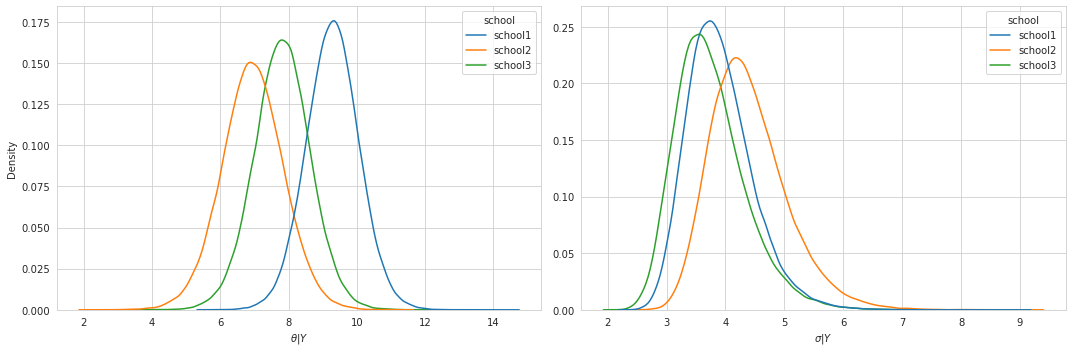
\includegraphics[width=0.9\textwidth]{5.1.a.png}
  \captionsetup{justification=centering}
  \caption{Posterior Distributions}
\end{figure*}

\paragraph{(a) Posterior Mean and Confidence Interval (CI)}
Note, according to the question, we are only showing the statistics for $\sigma|Y$, the posterior standard deviation, instead of the variances.
\begin{center}
\begin{tabular}{||c c c c c||} 
 \hline
 School & $\theta|Y$ mean & $\theta|Y$ 95\% CI & $\sigma|Y$ mean & $\sigma|Y$ 95\% CI \\ [0.5ex] 
 \hline\hline
 1 & 9.29 & (7.77, 10.82) & 3.91 & (3.00, 5.18) \\ 
 \hline
 2 & 6.94 & (5.14, 8.73) & 4.39 & (3.35, 5.88) \\
 \hline
 3 & 7.81 & (6.17, 9.45) & 3.75 & (2.80, 5.13) \\
 \hline
\end{tabular}
\end{center}

\paragraph{(b) Posterior $\theta_i < \theta_j < \theta_k$ Permutations}
\begin{center}
\begin{tabular}{||c c c c||} 
 \hline
 i & j & k & Prob($\theta_i<\theta_j<\theta_k)$ \\ [0.5ex] 
 \hline\hline
 1 & 2 & 3 & 0.00572 \\ 
 \hline
 1 & 3 & 2 & 0.00368 \\
 \hline
 2 & 1 & 3 & 0.08407 \\
 \hline
 2 & 3 & 1 & 0.67347 \\
 \hline
 3 & 1 & 2 & 0.01517 \\
 \hline
 3 & 2 & 1 & 0.21789 \\
 \hline
\end{tabular}
\end{center}

\paragraph{(c) Posterior $\tilde{Y}_i < \tilde{Y}_j < \tilde{Y}_k$ Permutations}
\begin{center}
\begin{tabular}{||c c c c||} 
 \hline
 i & j & k & Prob($\tilde{Y}_i < \tilde{Y}_j < \tilde{Y}_k)$ \\ [0.5ex] 
 \hline\hline
 1 & 2 & 3 & 0.10624 \\ 
 \hline
 1 & 3 & 2 & 0.10467 \\
 \hline
 2 & 1 & 3 & 0.18327 \\
 \hline
 2 & 3 & 1 & 0.26838 \\
 \hline
 3 & 1 & 2 & 0.13745 \\
 \hline
 3 & 2 & 1 & 0.19999 \\
 \hline
\end{tabular}
\end{center}

\paragraph{(d) Posterior Probability for School 1 vs. Others}
The posterior probability that $\theta_1|Y$ is bigger than both $\theta_2|Y$ and $\theta_3|Y$ is 0.89136.
And the posterior probability that $\tilde{Y}_1|Y$ is bigger than both $\tilde{Y}_2|Y$ and $\tilde{Y}_3|Y$ is 0.46837.

\paragraph{Appendix}
The code for generating the posterior samples is included here for completeness.
\begin{lstlisting}[language=Python]
import pandas as pd
import numpy as np
import seaborn as sns
import matplotlib.pyplot as plt
import scipy.stats as stats

sns.set_style('whitegrid')

# read in the data
file_names = ["school1.dat", "school2.dat", "school3.dat"]

dfs = []
for i, fnm in enumerate(file_names):
    d = pd.read_table(fnm, header=None, names=['time'])
    d['school'] = fnm.split('.')[0]
    dfs.append(d)

df = pd.concat(dfs).reset_index(drop=True)

# priors parameters
mu0 = 5
kappa0 = 1
v0 = 2
sigma0_sq = 4

# school sufficient statistics
gp = df.groupby('school')
ns = gp.time.size()
y_bars = gp.time.mean()
vars = gp.time.var()

# posterior parameters
kns = kappa0 + ns
muns = (kappa0*mu0 + ns*y_bars) / kns
vns = v0 + ns
sigmans_sq = 1/vns * ((ns-1)*vars + v0*sigma0_sq + (kappa0*ns/kns)*(y_bars-mu0)**2)


np.random.seed(12123)

# drawing precision samples
precision_samples = stats.gamma(a=vns/2, scale=2/(vns*sigmans_sq)).rvs(size=(100000, 3))
vars_samples = 1 / precision_samples

# drawing mu samples given the precision samples
theta_samples = stats.norm(loc=muns, scale=np.sqrt(vars_samples/kns.values)).rvs()
\end{lstlisting}


\section{Exercise 5.2}
First, we know our data sample size for each group is 16. While we are using normal conjugate pairs, it also uses Bayesian shrinkage based on the relative weights between prior and observation sample sizes. With $\kappa_0$ and $\nu_0$ closer to 0, we put our belief more on the observations, group B on average, $\bar{y}_B=77.5$, is large than group A $\bar{y}_A=75.2$. On the other hand, if we think $\kappa_0$ and $\nu_0$ are large, it is equivalent to thinking that both groups come from the same population and that the observed differences are merely a sampling error.
\begin{figure*}[!h]
  \centering
  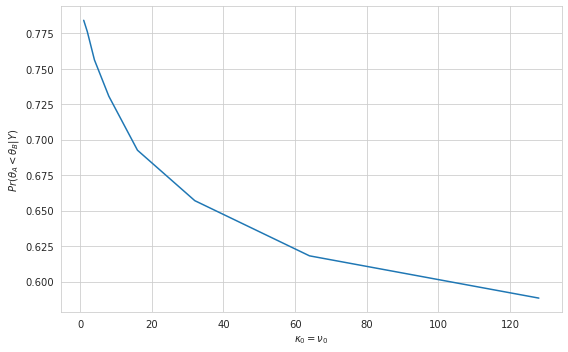
\includegraphics[width=0.55\textwidth]{5.2.a.png}
  \captionsetup{justification=centering}
  \caption{Sensitive Analysis using Monte Carlo on Normal conjugates}
\end{figure*}

\paragraph{Appendix}
The code for generating the posterior samples is included here for completeness.
\begin{lstlisting}[language=Python]
import pandas as pd
import numpy as np
import seaborn as sns
import matplotlib.pyplot as plt
import scipy.stats as stats

sns.set_style('whitegrid')

np.random.seed(12123)
sample_size = 100000

ps = []
for epoch in range(8):
    # priors parameters
    kappa0, v0 = 2**epoch, 2**epoch
    mu0 = 75
    sigma0_sq = 100

    # group sufficient statistics
    ns = np.array([16, 16])
    y_bars = np.array([75.2, 77.5])
    vars = np.array([7.3, 8.1])**2

    # posterior parameters
    kns = kappa0 + ns
    muns = (kappa0*mu0 + ns*y_bars) / kns
    vns = v0 + ns
    sigmans_sq = 1/vns * ((ns-1)*vars + v0*sigma0_sq + (kappa0*ns/kns)*(y_bars-mu0)**2)

    # drawing precision samples
    precision_samples = stats.gamma(a=vns/2, scale=2/(vns*sigmans_sq)).rvs(size=(sample_size, 2))
    vars_samples = 1 / precision_samples

    # drawing mu samples given the precision samples
    theta_samples = stats.norm(loc=muns, scale=np.sqrt(vars_samples/kns)).rvs()

    ps.append((theta_samples[:,0] < theta_samples[:,1]).mean())
\end{lstlisting}


\section{Exercise 6.1}
\paragraph{(a) Prior Distribution Setup}
We are provided with the following assumption that $\theta_A = \theta$, $\theta_B = \theta \times \gamma$, where $\theta \thicksim Gamma(a_\theta, b_\theta)$ and $\gamma \thicksim Gamma(a_\gamma, b_\gamma)$. Hence, $\theta_A$ and $\theta_B$ are only conditional independent given the parent $\theta$. The $\gamma$ parametrization doesn't play a role in the dependency chain here. The justification for such a setup is straightforward. Perhaps we think the two group shares some similarities from a common population.
\begin{align*}
    p(\theta_A, \theta_B|\theta) = p(\theta_A|\theta) \times p(\theta_B|\theta)
\end{align*}

\paragraph{(b \& c) Full Conditionals}
\begin{align*}
    p(y_A|\theta_A) &= \prod_i(\frac{1}{y_{iA}!}) \theta^{n_A\bar{y_A}} e^{-n_A\theta} \\
    p(y_B|\theta_B) &= \prod_i(\frac{1}{y_{iB}!}) (\theta\gamma)^{n_B\bar{y_B}} e^{-n_B\theta\gamma} \\
        &= \prod_i(\frac{1}{y_{iB}!}) \theta^{n_B\bar{y_B}} \gamma^{n_B\bar{y_B}} e^{-n_B\theta\gamma} \\
    p(\theta) &= \frac{b_{\theta}^{a_\theta}}{\Gamma(a_{\theta})} \theta^{a_\theta-1} e^{-b_\theta \theta}
        && \theta \thicksim Gamma(a_\theta, b_\theta) \\
    p(\gamma) &= \frac{b_{\gamma}^{a_\gamma}}{\Gamma(a_{\gamma})} \gamma^{a_\gamma-1} e^{-b_\gamma \gamma}
        && \gamma \thicksim Gamma(a_\gamma, b_\gamma) \\ \\
    p(\theta|y_A, y_B, \gamma) &\propto p(\theta, y_A, y_B, \gamma) \\
        &\propto p(y_A|\theta) p(y_B|\theta, \gamma) p(\theta) \\
        &\propto \theta^{a_\theta + n_A\bar{y_A} + n_B\bar{y_B} - 1} \exp[-\theta(n_A+n_B\gamma+b_\theta)] \\
    \theta|Y, \gamma &\thicksim Gamma(a_\theta + n_A\bar{y_A} + n_B\bar{y_B}, b_\theta+n_A+n_B\gamma) \\ \\
    p(\gamma|y_A, y_B, \theta) &\propto p(y_A, y_B|\theta, \gamma) p(\gamma) p(\theta) \\
        &\propto p(y_B|\theta, \gamma) p(\gamma) \\
        &\propto \gamma^{a_\gamma + n_B\bar{y_B}-1} \exp[-\gamma(b_\gamma + n_B\theta)] \\
    \gamma|Y, \theta &\thicksim Gamma(a_\gamma + n_B\bar{y_B}, b_\gamma + n_B\theta)
\end{align*}

\paragraph{(d) Gibbs Sampler}
Here we did a quick, sensitive analysis on $\gamma$. By setting the prior parameter $a_\gamma = b_\gamma$, we started with our prior assumption that the mean of $\gamma$ is 1, $\mathbf{E}[\gamma] = \frac{a_\gamma}{b_\gamma}$ because it is a gamma distribution. Furthermore, we parameterized $\theta_A = \theta$ and $\theta_B = \theta \times \gamma$ as such. $\gamma$ is the relative rate of group A and group B. The larger the two prior parameters, the stronger the prior belief that $\gamma$ is 1. Its precisely what we see in Figure 3. 
\begin{figure*}[!h]
  \centering
  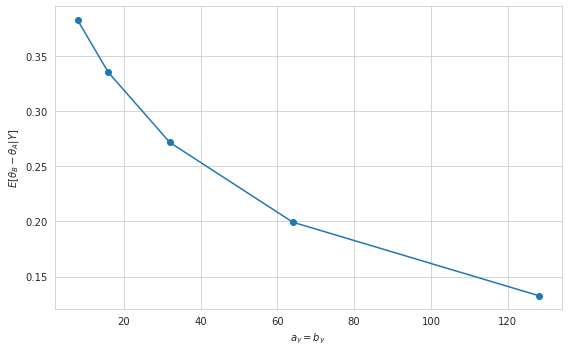
\includegraphics[width=0.55\textwidth]{6.1.d.png}
  \captionsetup{justification=centering}
  \caption{Sensitive Analysis using Gibbs Sampler}
\end{figure*}

\newpage
\paragraph{Appendix}
Here is the code for the Gibbs sampler that I used for this problem.
\begin{lstlisting}[language=Python]
import pandas as pd
import numpy as np
import seaborn as sns
import matplotlib.pyplot as plt
import scipy.stats as stats

sns.set_style('whitegrid')

def read_bach_file(fnm):
    data = []
    with open(fnm, "r") as t:
        for line in t.readlines():
            d = line.strip()
            if d == '': continue
            data.extend(list(map(int, d.split(' '))))
    return np.array(data)
    
bach = read_bach_file("menchild30bach.dat")
nobach = read_bach_file("menchild30nobach.dat")

burnin = 1000
epochs = 10000
target_stats = []

# observation data sufficient statistics
nA, mean_yA = bach.shape[0], bach.mean()
nB, mean_yB = nobach.shape[0], nobach.mean()

# for each gamma prior pair
for i in range(5):
    samples = []

    # prior parameter setup
    a$\theta$, b$\theta$ = 2, 1
    a$\gamma$, b$\gamma$ = 2**(i+3), 2**(i+3)

    # initial sample setup
    $\theta$, $\gamma$ = 1.3, 1
    for epoch in range(burnin+epochs):
        # sample from the full conditionals
        $\theta$_fullcond = stats.gamma(a=a$\theta$+nA*mean_yA+nB*mean_yB, scale=1/(b$\theta$+nA+nB*$\gamma$))
        $\theta$ = $\theta$_fullcond.rvs()

        $\gamma$_fullcond = stats.gamma(a=a$\gamma$+nB*mean_yB, scale=1/(b$\gamma$+nB*$\theta$))
        $\gamma$ = $\gamma$_fullcond.rvs()

        samples.append(($\theta$, $\gamma$))

    # calculate the expectation from the samples
    df = pd.DataFrame(samples[burnin:], columns=['theta','gamma'])
    df['theta_B'] = df.theta * df.gamma
    s = (df.theta_B - df.theta).mean()
    target_stats.append(s)
\end{lstlisting}

\end{document}